This section describes case study as the chosen research method for the study. Yin defines a case study in the following way \cite{CaseStudyResearch}:

\begin{enumerate}
\item A case study is an empirical inquiry that
\begin{itemize}
\item investigates a contemporary phenomenon in depth and within its real-life context, especially when
\item the boundaries between a phenomenon and context are not clearly evident.
\end{itemize}
\item The case study inquiry
\begin{itemize}
\item copes with the technically distinctive situation in which there will be many more variables of interest than data points, and as one result
%Hva er variables og hva er data points?
\item relies on multiple sources of evidence, with data needing to converge in a triangulating fashion, and as another result
\item benefits from the prior development of theoretical propositions to guide data collection and analysis.
\end{itemize}
\end{enumerate}

The research process is illustrated in figure \ref{fig:caseProcess}. As the figure shows, the process in linear, but iterative. This means that one can go back to previous phases if one sees the need for that. The Plan phase consisted of identifying research questions and deciding to use case study as the research method for this study. The Design phase is about getting from initial questions to conclusions or answers. It is the logic that links the data to be collected to the initial questions of the study \cite{CaseStudyResearch}. 

\begin{figure}[H]
\begin{center}
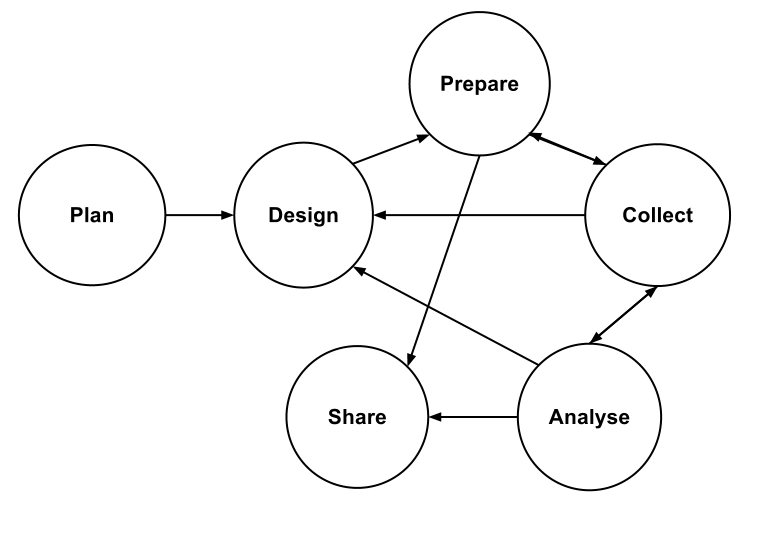
\includegraphics[scale=0.38]{caseProcess.png}
\caption[Case Study Research Process]{Case Study Research Process \cite{CaseStudyResearch}}
\label{fig:caseProcess}
\end{center}
\end{figure}

%The case design has five important components \cite{CaseStudyResearch}:

%\begin{enumerate}
%\item A study's questions
%\item Its propositions, if any
%\item Its unit(s) of analysis
%\begin{enumerate}
%\item What is the case?
%\end{enumerate}
%\item The logic linking the data to the propositions
%\begin{enumerate}
%\item analytic techniques, should be known prior to the data collection, so the right data will be collected
%\end{enumerate}
%\item The  criteria for interpreting the findings
%\begin{enumerate}
%\item The challenge is to anticipate and enumerate the important rival explanations for the findings
%\end{enumerate}
%\end{enumerate}

%These components were identified in the Design phase and each case and its design is described further in chapter \ref{chp:CaseIntroductions}.

Yin presents tactics to maximize the quality of empirical research \cite{CaseStudyResearch}. It is recommended to use multiple sources of evidence and to have key informants review a draft of the report. Both of these tactics were used in this study. %These tactics are applied to four different tests as shown in figure \ref{fig:caseTactics}. The test for internal validity is not so relevant for this study, as it is mainly an \textit{exploratory} study.


%\begin{figure}[ht]
%\begin{center}
%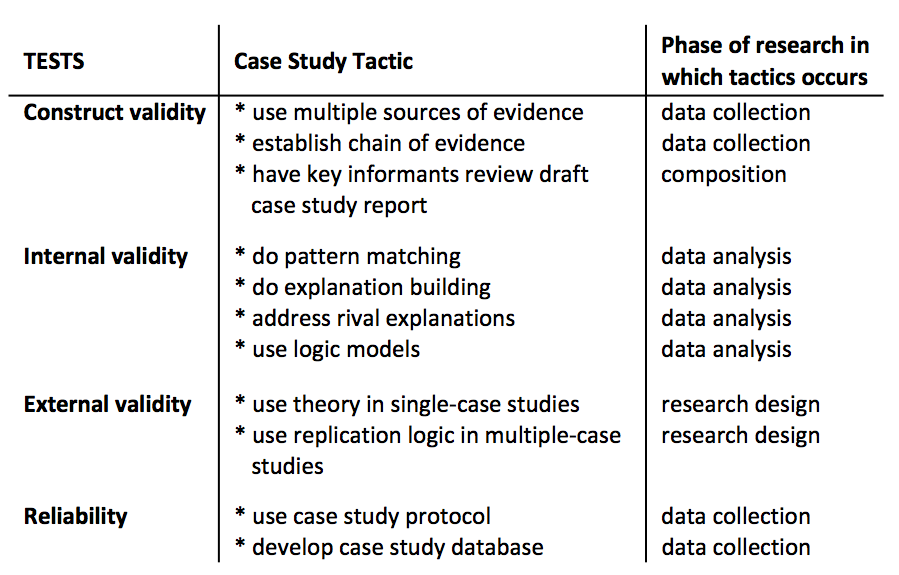
\includegraphics[scale=0.82]{caseTactics.png}
%\caption[Case Study Tactics for Four Design Tests]{Case Study Tactics for Four Design Tests %\cite{CaseStudyResearch}}
%\label{fig:caseTactics}
%\end{center}
%\end{figure}

The choice between a single- and multiple-case belongs to the Design phase. Multiple-case is usually preferred and was chosen as the method for this study. Additionally each case may be embedded or holistic. An embedded case has more than one unit of analysis. The design for this study is a mix, a multiple-case with one embedded case and two holistic cases. %NB, dette kan endres!!!! Multiple: select each case so that it either (a) predicts similar results (literal replication) or (b) predicts contrasting results but for anticipatable reasons (theoretical replication). Dette har vel ikke vi gjort
The design is illustrated in figure \ref{fig:caseDesign}.

\begin{figure}[ht]
\hspace{-0.28cm}\includegraphics[scale=0.375]{caseStructure.png}
\caption[Case Design for This Study]{Case Study Design, modified from \cite{CaseStudyResearch}}
\label{fig:caseDesign}
\end{figure}

The Preparation phase was very important as we did not have experience with the case study research method. The main activities performed in this phase were acquiring desired skills to become case study investigators and preparing for the specific case studies. It is considered difficult to obtain these skills as procedures are not routinised. It is advised to prepare to ask good questions, be a good "listener", be adaptive and flexible, have a firm grasp of the issues being studied and be unbiased by preconceived notions \cite{CaseStudyResearch}. We have performed a background study in order to get a thorough understanding of the issues in the study. Relevant background information is discussed in chapter \ref{chp:background} and the background study itself is briefly discussed in section \ref{sec:background}. %Develop a protocol for the investigation? screen candidate cases? Pilot case? No..

Interviews, documents and surveys were chosen as the sources of information in the Collection phase. The use of multiple sources of evidence is consistent with the definition of a case study, which is presented in the beginning of this section. The interview is seen as being one of the most important sources of information in a case study \cite{CaseStudyResearch}. Documentary information is likely to be relevant in any case study \cite{CaseStudyResearch}. These data collection methods are described and discussed in sections \ref{sec:interviews}, \ref{sec:documentStudy} and \ref{sec:employeeSurveys}.

The Analyse phase is described in section \ref{sec:qualitativeAnalysis}.

The Share phase consisted of preparation, writing and editing this report. Choices such as to anonymize identities of individuals and individual organizations were a part of this phase. This choice is further discussed in section \ref{sec:ethical}. It was a choice that was made as part of the preparation of the study and this illustrates the arrow from Prepare directly to Share, and shows that the case study process is not purely linear. 